\subsection{Overview: Result Clustering}
CubanSea is the name chosen for the implemented visualization interface prototype. It abbreviates ``\underline{c}l\underline{u}ster-\underline{ba}sed visualizatio\underline{n} of \underline{sea}rch results''. Instead of an ordered result list, the CubanSea interface returns a set of distinguishable areas, each containing a subset of the total result list. These subsets are overlapping and cover the entire total result list. Each area corresponds to one topic occuring in the result space. Figure \ref{fig:overview:piracy} displays the visualization generated when searching for ``piracy''. As you can see, two different topics have been identified: ``software pirates report'' obviously refers to software piracy, or piracy of digital media in general, while ``pirates history robbery'' talks about historic sea robbery. These topic headers have been automatically generated and provide the viewer with the ability to immediatly grasp the topic space.
\begin{figure*}[!t]
	\centering
	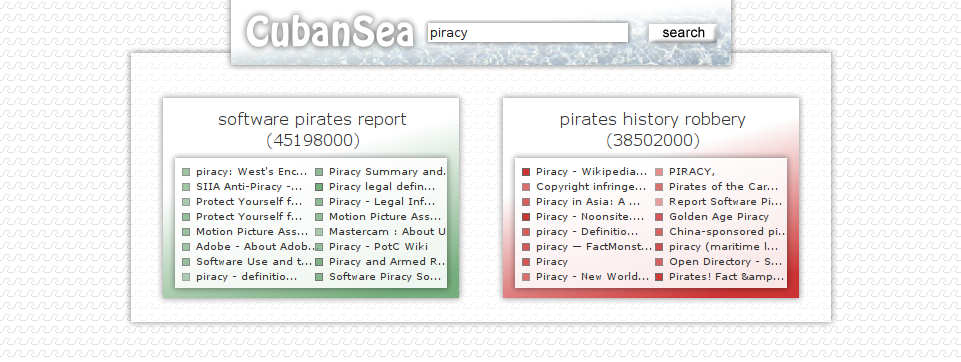
\includegraphics[width=6.5in]{cubansea-overview_piracy}
	\caption{Clusters generated for the query ``piracy''}
	\label{fig:overview:piracy}
\end{figure*}
Aiming to increase percivability, each topic is being encoded with a distinct color. These colors have been chosen in accordance to \cite{Berlin1969}, identifying green, red, blue, and yellow as being the most effective color set for labeling. Since yellow has a very low luminance contrast to the white background, it has been replaced with a dark grey. In order to prevent using high volume colors on large areas which would distract the viewers attention as pointed out in \cite{Ware2004}, a light gradient has been chosen. This gradient is enough to convey a basic understanding of the cluster colors to the user without taking the attention from the content. The top 20 results of each cluster are provided to aid the in topic recognition in the event that the headers might be ambiguous. The results are printed on a white-faded background to counter the interfering effect gradient background has on text.

The CubanSea interface only provides the visualization of search results. The results themselves are being retrieved from a search engine provider. For the purpose of this paper, the Yahoo Search API \cite{YahooSearchAPI} has been chosen. However, the system is designed to work with any search engine. In order to generate the visualization, an initial amount of search results has to be retrieved from the search engine provider. The number of this initial retrieval is critical to the success of CubanSea. As mentioned before, performance is a vital aspect for search engine interfaces. Fetching results from the search engine provider requires a number of network connections, thus posing a bottleneck for the entire application. The fewer search results are initially retrieved, the better the performance of the system. However, clusters construction yields better results when a larger data set is being used. Hence, it is necessary to balance number of initially requested results to achieve the optimal mixture of performance and cluster quality. During my experiments, 50 results has proven to be a reasonable amount.

After retrieving the initial search results from the provider, it is necessary to convert these results into multi-dimensional vectors that can be processed by clustering algorithms. \cite{Hoeber2006a} provides a successful solution for this, using the \emph{Porter Suffix Striping Algorithm} presented in \cite{Porter1997} to calculate the number of occurrences of different term-stems inside the result documents. \cite{Rauber2000} suggests additionally multiplying these occurrences with the inverse document frequency. However, applying this proved no significant increase in the quality of the results. I therefore decided against it, favoring performance increase. Search engines typically return only a short summary of the result documents, called ``snippets''. Retrieving all original documents prior to performing the clustering would require 50 network connections. Since this would be a significant lack in performance, it is more feasible to use the snippets for constructing the multi-dimensional vectors. Initial experiments to also consider the title of the document resulted in unsatisfactory results. It can be hypothesized, that this is due to the fact that too many titles use the same set of words such as ``overview'', ``home'', or ``results''. Snippets, however, display the actual context of the term's utilization inside the document. Hence, it is likely to be more relevant and meaningful in respect to the query.
\begin{figure*}[!t]
	\centering
	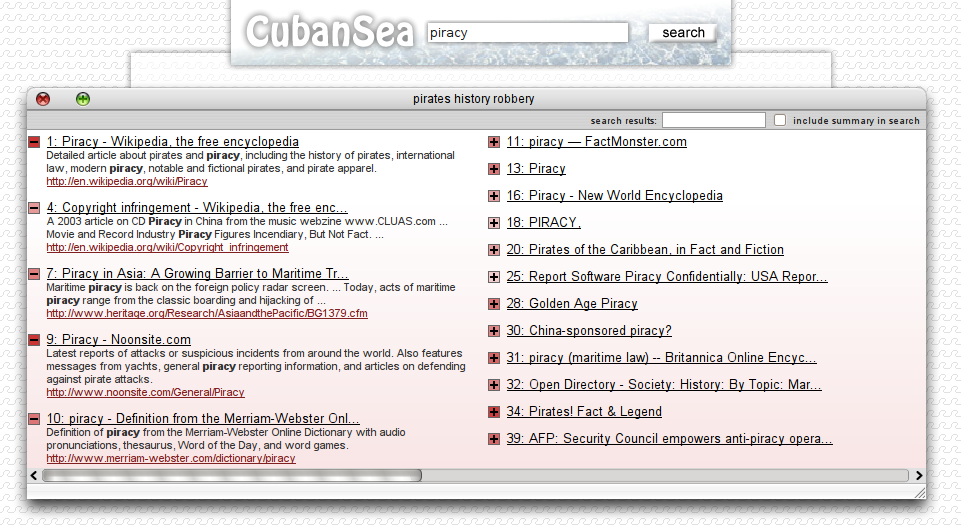
\includegraphics[width=6.5in]{cubansea-zoom_piracy}
	\caption{Displaying the ``pirates history robbery'' cluster}
	\label{fig:zoom:piracy}
\end{figure*}

For the clustering algorithm I have chosen the \emph{Fuzzy-C-Means Algorithm} discussed in \cite{Dunn1973} and \cite{Bezdek1981}. This algorithm iteratively calculates a predefined amount of centroids in a multi-dimensional space and evaluates the membership of the individual items to these centroids using the formula in equation \ref{eq:cluster:membership} where $u_{ij}$ is the membership value of result $i$ in cluster $j$. While $x_i$ represents the multi-dimensional vector of result $i$, $c_j$ holds the vector representing the centroid of cluster $j$. $m$ is a so called ``fuzzifier'' determining the crispness of the clusters. \cite{Stutz1999} shows a fuzzifier between 1 and 2.5 to be most effective. For this application, 1.5 has proven to be a reasonable choice. $|c|$ denotes the number of clusters.
\begin{equation}
	u_{ij} = \left(\displaystyle\sum_{k=0}^{|c|} \left(\frac{\|x_i - c_j\|}{\|x_i -c_k\|}\right)^{\frac{2}{m-1}}\right) ^{-1} \label{eq:cluster:membership}
\end{equation}
Generally, any kind of distance function can be used for $\|x_i - c_j\|$ in this equation. Due to simplicity, the eucledian distance  was chosen for CubanSea. Each iteration optimizes the centroids and recalculates the membership values. As soon as this optimization does not yield a significant change, the algorithm terminates, returning the current centroids as the resulting centers of the clusters.

The primary goal of this clustering is to provide the user with some kind of overview over the result space. This overview is helpful since the human mind is limited in how many objects he can preattentive process \cite{Healey1996}. Obviously, it would be counterproductive to generate more clusters than that number. My experiments have shown four to be an effective number of clusters to be generated by the algorithm, lying well below the suggested maximum of 5-10. Clearly, it cannot be assumed that the result space always consists of exactly that many distinct topics. Hence, by configuring the clustering algorithm, we intentionally restrict the visualization to display only the four most relevant clusters. In case that there are actually less than four distinct topics, the cluster centroids will lie close to each other. By simply merging all clusters with a distance to each other less than a certain minimum, the cluster set can be reduced to those actually representing distinct and meaningful topics.

After generating the different topics, the results now have to be assigned to the different clusters. For this, a minimal membership is defined. Results are assigned to all those clusters in which they have a membership equal or higher to the minimal membership. In case that a result is not assigned to any cluster this way, it is simply added to the cluster it has the highest membership in. The number of total results for a cluster as displayed in figure \ref{fig:overview:piracy} can be interpolated by multiplying how many percent of the retrieved results are assigned to a cluster with the estimated total number of results provided by the search engine provider.

Finally, the topic headers must be determined. The headers are constructed using the most frequently used keywords occuring in the topics. Each cluster centroid consists of a multi-dimensional vector recording the number of occurrences of the different word stems. Identifying the three most frequently occurring stems is trivial. However, word stems are no regular words and thus using them can be obstrusive. This problem can be resolved by determining for each stem the most frequent word containing the stem inside the result documents. Naturally, the search terms should be ignored in this process since they are likely to appear frequently in all clusters. Their use would diminish the unambiguity of the headers. This process does not guarantee to generate unambiguous topic headers, but provides a good starting point and the results are sufficient for this application.

\begin{figure*}[!t]
	\centering
	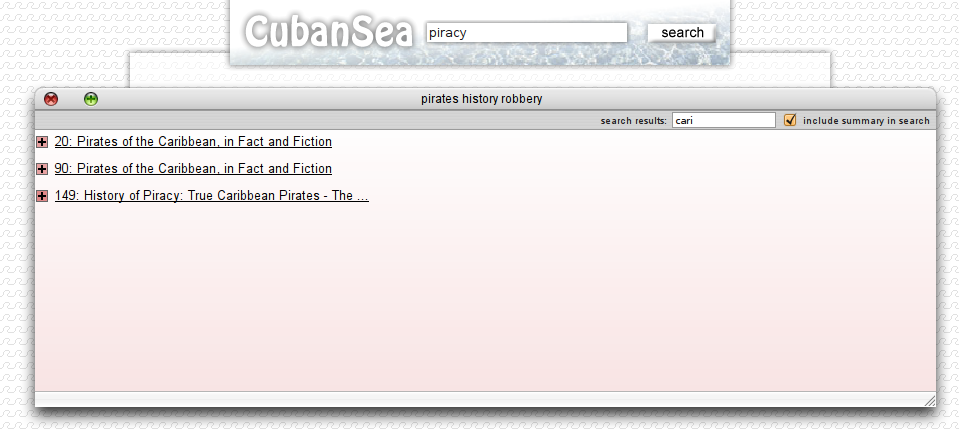
\includegraphics[width=6.5in]{cubansea-filter_piracy}
	\caption{Filtering the result space using ``cari''}
	\label{fig:filter:piracy:cari}
\end{figure*}